\newpage
\subsection{Actividad 16}
Diseñar un controlador vector de ganancias en espacio de estado
continuo para que el sistema en bucle cerrado en velocidad presente un
par de polos deseados con comportamiento críticamente amortiguado y
exhiba una frecuencia natural de $\omega_n$ de 10, asegurando error nulo ante
consigna velocidad con amplitud unitaria, partiendo de condiciones
iniciales nulas y especificando el resto de polos deseados a
suficiente distancia de los anteriores. Asumir que el estado es
observable. Posteriormente, graficar la respuesta del sistema de
control en velocidad en \textsc{MATLAB}.

Aunque \textsc{MATLAB} nos proporciona un modelo en el espacio de
estados para el sistema de velocidad hemos preferido hacerlo a mano
para seleccionar un vector de estado lógico (respecto a las variables
físicas que queremos controlar).

\begin{equation}
  \begin{split}
    \dfrac{V_s(s)}{V_e(s)} &= \dfrac{0.00544}{3.456\cdot10^{-5}s^2+0.002386s+0.01207}\\
    0.00544V_e(s) &= 3.456\cdot10^{-5}V_s(s)s^2+0.002386V_s(s)s+0.01207V_s(s)\\
    0.00544V_e(t) &=
    3.456\cdot10^{-5}V_s''(t)+0.002386V_s'(t)+0.01207V_s(t)\\
  \end{split}
\end{equation}
Seleccionamos como vectores de estado la velocidad y la
aceleración.
\begin{equation}
  \begin{split}
    x_1 &= V_s \ \ \ \ \ \ \ \ \dot x_1 = V_s' = x_2\\
    x_2 &= V_s' \ \ \ \ \ \ \ \ \dot x_2 = V_s''
    \end{split}
  \end{equation}
\begin{equation}
  \begin{split}
0.00544 u &=  3.456 \cdot 10^{-5} \dot x_2 + 0.002386 x_2 + 0.01207 x_1\\
\dot x_2 &= 157.4074 u - 69.0394x_2-349.2477x_1\\
\end{split}
\end{equation}

\begin{equation}
  \begin{bmatrix}
    \dot x_1 \\
    \dot x_2
\end{bmatrix} =
\begin{bmatrix}
  0 & 1\\
  -349.2477 & -69.0394
\end{bmatrix}
\begin{bmatrix}
  x_1\\
  x_2
\end{bmatrix}
+
\begin{bmatrix}
  0\\
  157.4074
\end{bmatrix}
\begin{bmatrix}
  u
\end{bmatrix}
\end{equation}

\begin{equation}
  y = 
  \begin{bmatrix}
1 & 0
\end{bmatrix}
\begin{bmatrix}
  x_1\\
  x_2
\end{bmatrix} 
\end{equation}

\newpage
\lstinputlisting[language=MATLAB]{./codes/actividad16.m}
\begin{tcolorbox}[sharp corners, colframe=bluebox, title= Respuesta
  del sistema en tiempo continuo]
 % $>>>$ ltiview(\textcolor{blue}{`lsim'},kr*feedback(PDI\_10*Gposicionz,kr))
  \vspace*{0.35em}
  \mkanscode{
\begin{figure}[H]
  \centering
  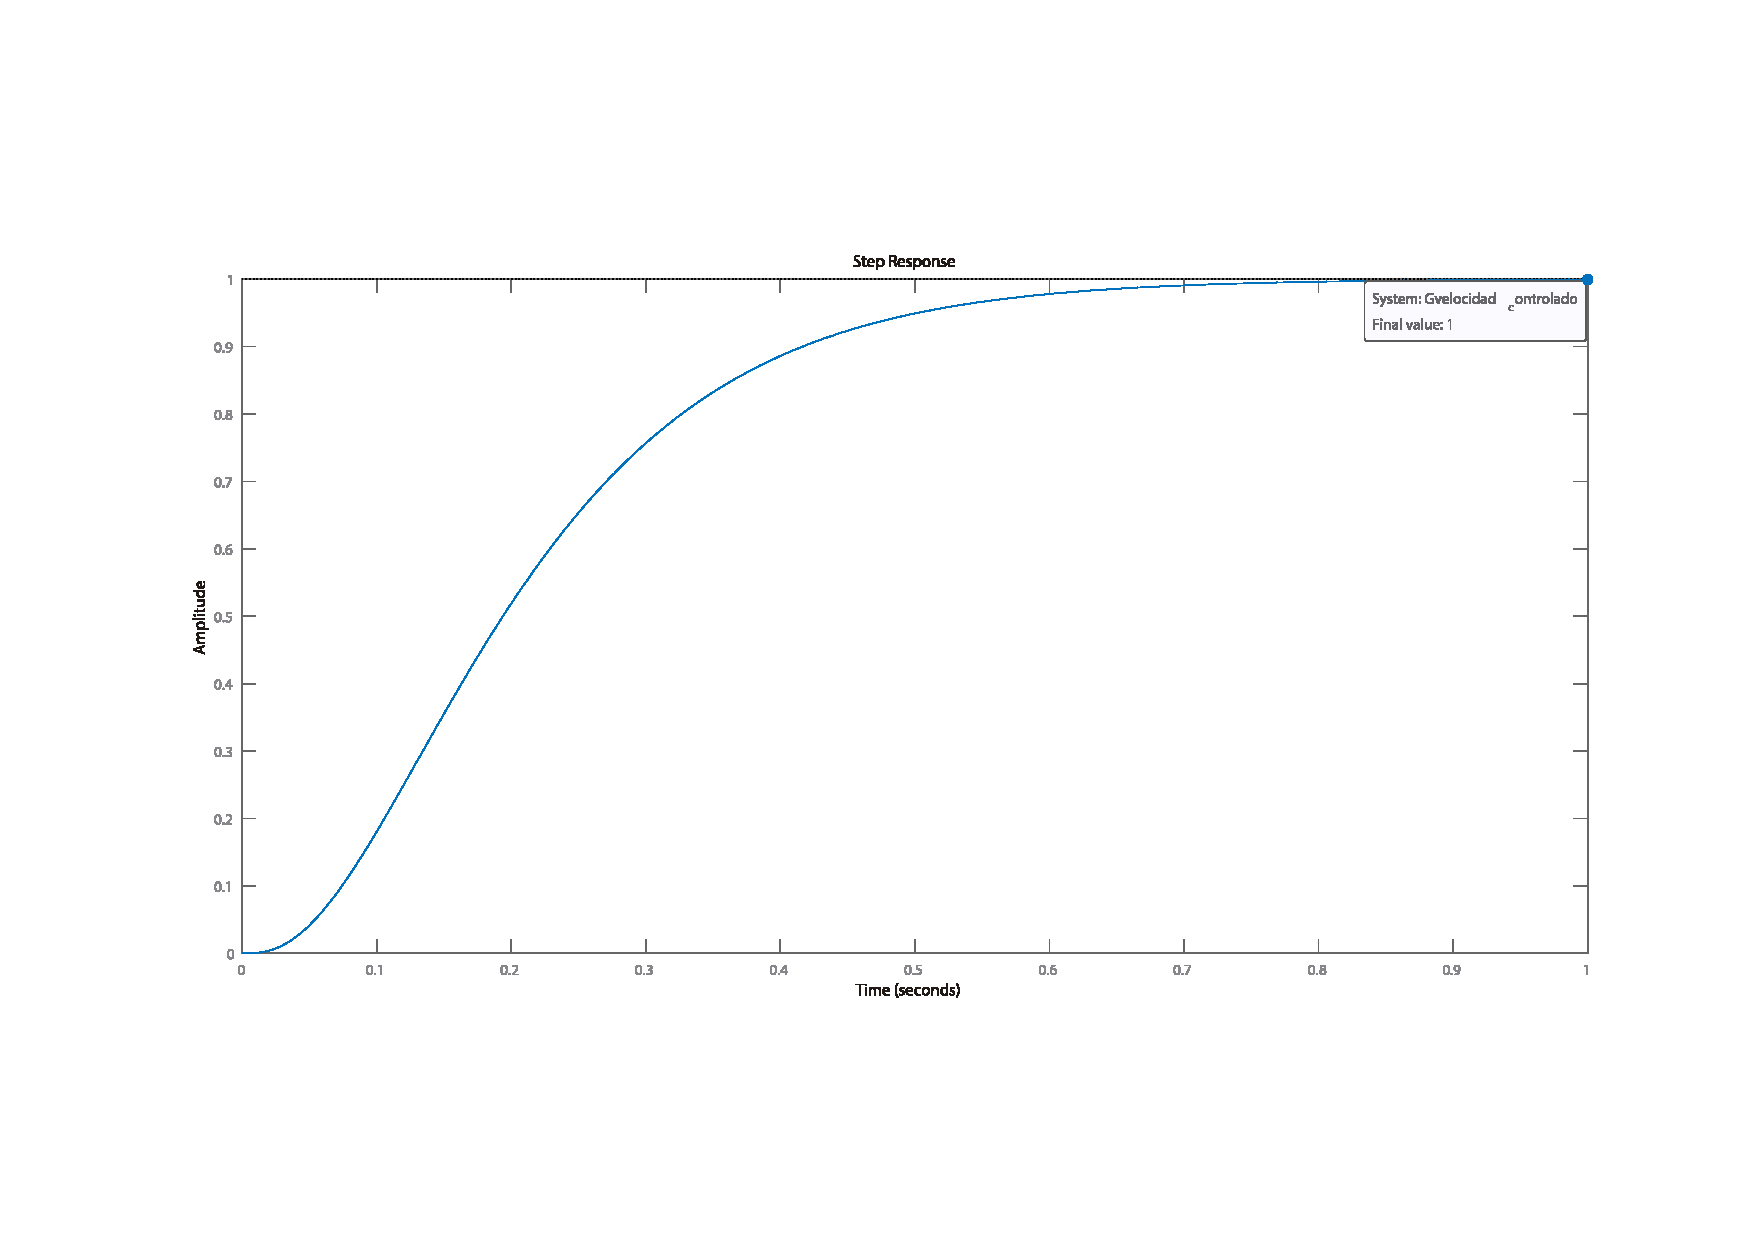
\includegraphics[clip, trim=2.5cm 4.5cm 2.5cm 4.25cm,
  scale=0.5]{images/figura 18.pdf}
  % izquierda,abajo,derecha,arriba
  \caption{Respuesta del sistema con error nulo.}
    \label{fig:figura 18}
\end{figure}
}
\vspace*{0.35em}
  \end{tcolorbox}%